\chapter{Methodology}
\label{chap:methodology}
In this chapter we explain how we implement the sketching schemes MinHash and FSS in Section \ref{section:minhash} and \ref{section:fss}. The sketches resulting from these schemes are fed to a LSH scheme. Implementation details of LSH are listed in Section \ref{section:lsh_implementation}. Section \ref{section:meth:amplification} proceeds with an extensive discussion on the implementation of amplified LSH schemes. We end the chapter by introducing the approach to evaluation of the methods in place in Section \ref{section:meth:evaluation_lsh_schemes}.

\section{Creating integer-based representations of the sets of model words}
\label{section:hashing}
The LSH algorithms of interest in this thesis, such as MinHash and FSS, aim to produce hashes which can be used to estimate a set similarity function on the input sets. Efficient implementations of these LSH algorithms use hash functions that require integer inputs. Hence, we need to map the elements in the original sets, which are string values, to an integer-based set representation. 

We use a function that takes as input strings and generates a $32$-bit integer output in $[2^{32}]$. To reiterate notation introduced in Section \ref{section:lit:applying_lsh_to_deduplication_of_docs_on_web}, $[n]$ represents the set ${0,1,...,n-1}$. The function starts by encoding the input in a binary utf-8 format. This encoded string is then fed to a SHA-1 hash function that generates a $20$ byte number. Since we only need a $32$-bit number, we take the first $4$ bytes and convert those back to an integer format. We apply this approach to each set of model words and store the resulting sets of integers. This approach does not lead to any collisions in our dataset.

\section{MinHash}
\label{section:minhash}
For the implementation of MinHash, we use the open source Python package \textit{datasketch}\footnote{available at https://github.com/ekzhu/datasketch}. To generate a sketch $S(X)$ of length $n$, we use $n$ universal hash functions of the form $h_{(a_i,b_i)}(x) = (a_i * x + b_i) \mod c \mod 2^{32}$, so that each $x \in X$ is hashed to a value in $[2^{32}]$. Notice that the$\mod 2^{32}$ operation is equivalent to preserving the last $32$ bits of $(a_i * x + b_i) \mod c$. For the parameter $c$ we use the Mersenne prime $2^{61} - 1$. $a_i$ and $b_i$ are both randomly drawn from $[c] = [2^{61} - 1]$. Then the $i$-th sketch value $S(X)[i] = \min_{x \in X}(h(a_i,b_i)(x))$.

\section{Fast Similarity Sketching}
\label{section:fss}
In Section \ref{section:lit:variations_minhash}, we concluded that FSS is the most worthy alternative to the MinHash scheme, promising both efficiency and effectiveness benefits. Hence, to answer the first research subquestion regarding the performance of alternative LSH schemes, we compare MinHash with FSS. For the implementation of FSS, we implement the fill-sketch algorithm as proposed by \cite{DahlgaardKT17} and extensively discussed in Section \ref{subsec:fss}.

For the random hash functions $h_0,...,h_{2n-1}$ we use two mixed-tabulation hashing functions, as introduced in Section \ref{subsec:mixed_tab}. A few modifications are made in order to achieve the $O(1)$ hash evaluation. Each mixed tabulation hashing function will hash $64-$bit integer inputs $q$, where $q$ is defined as the binary concatenation of $x$ and $i$, both represented as $32-$bit integers. Since we use $64$-bits inputs, the size of T1 is increased to $256 \times 8$. In step $2$ of the algorithm the input $q$ is then split in $8$ $8$-bit parts instead of $4$. The rest of the algorithm proceeds as laid out in Section \ref{subsec:mixed_tab}. With this approach, the hash tables T1 and T2 need only be generated once to generate $2n$ random hashes. As mentioned earlier, we use two mixed tabulation hashing functions. The hash output $h_{1i}$ of the first mixed tabulation hashing function is used to generate $v_i(x)$
\begin{equation}
    v_i(x) = \frac{h_{1i}}{2^{32} - 1}
\end{equation}
The hash output $h_{2i}$ of the second mixed tabulation hashing function is used to generate $b_i(x)$
\begin{equation}
    b_i(x) = \begin{cases} h_{2i} \mod n \text{          , if  } i<n\\
        i \text{         , if  } i>= n
    \end{cases}
\end{equation}

An out-of-the-box implementation of mixed tabulation hashing in the programming language \verb!C++! has been created by \cite{mixedTabimplementDahlgaard}. We have written Python bindings in order to be able to use the functionality in our implementation. 

\section{Implementation of LSH algorithm}
\label{section:lsh_implementation}
For the implementation of the traditional LSH algorithm we use the MinHashLSH class provided by the aforementioned \textit{datasketch} package. Contrary to its naming, this class is not only applicable to MinHash sketches, but also to other types of sketches such as FSS sketches. This class implements the original LSH algorithm as proposed by \cite{IndykM98}. When an LSH object from the class is initialized, a list of $b$ hash tables is generated. Each hash table is empty initially. The keys of each hash table have a length of $r$. 

We then add the sketches from our sketching scheme to the LSH object. Each sketch is divided into $b$ parts of length $r$. For each part $j$, we check in the corresponding hash table in the list of hash tables whether a hashcode has been generated which is equal to part $j$. If that is the case, then the corresponding data point $p$ is attached to the set of values already attached to that hashcode. If that is not the case, then a new key-value pair is initialized with as key part $j$ and as value a set containing the data point $p$

After all sketches have been added to the LSH object, we can extract the candidate pairs. The \textit{datasketch} package at the moment does not have a function for that goal, so we have written our own implementation. First, an empty set $C$ is initialized. Then, an iteration through the hash tables is started. In each hash table, candidate pairs $(p,p')$ are extracted from the hashcodes that have more than one data point $p$ attached. These candidate pairs are added to $C$. After all hash tables have been visited, we return $C$, which contains all candidate pairs.

\section{Amplification of LSH schemes}
\label{section:meth:amplification}
In Section \ref{section:lit:amplifying} we introduced the concept of amplification. To answer the second research subquestion, we need to implement and evaluate an amplified LSH scheme. In this section we introduce a new mathematical framework for analyzing amplified LSH schemes. Using this mathematical framework, we prove that an amplified LSH scheme is theoretically guaranteed to perform as well as traditional LSH schemes, while very likely to outperform traditional LSH schemes in practice. Then we provide an algorithm that can obtain optimal parameter values for both amplified and non-amplified LSH schemes. We end this section by providing implementation details of the amplified LSH scheme, most importantly introducing an algorithm which can be used to extract candidate pairs.

\subsection{Visualization of LSH scheme}
Using the example of a traditional LSH scheme, we introduce a visual structure, which helps us analyze the proposed amplified LSH schemes. Figure \ref{fig:lsh_traditional_visualization} provides a visualization of such a scheme, in this case with $r=4$ and $b=4$, making for a total of $16$ hash functions $h_i(\cdot)$. For an imaginary pair of inputs $(p, p')$, we have created numbered circles that represent whether hash function $h_i(\cdot)$ produces equal output for $p$ and $p'$. If the circle is colored green, then we know that $h_i(p) = h_i(p')$, while a red color indicates that $h_i(p) \neq h_i(p')$. As $r=4$, we find that each group of $4$ consecutive hash functions $h_i$ is connected with AND operators. The AND operators indicate that we need all $4$ functions $h_i$ to produces the exact same output, in order for a positive (candidate) signal to be produced. $b=4$ on the other hand indicates that there are $4$ such groups $g_j(p)$ of hash functions. In the visualized structure these are connected via OR operators, indicating that a positive signal from one of the groups would be sufficient for a positive (candidate) signal. Following these rules, we can conclude that the visualized structure on the left represents a pair of inputs $p, p'$ that is a candidate pair. This is straightforward to see, as all circles are colored green in the second band. Mathematically, we say that $h_i(p)=h_i(p'), \text{ } \forall i \in [5,8]$, and $g_2(p) = g_2(p')$, which means that $p$ and $p'$ are assigned to the same bucket with hash value $g_2(p)$. This is not the case in the visualized structure on the right, although the same total number of hash functions agree.  Here none of the $4$ groups of hash functions produce a positive signal, implying that $p$ and $p'$ are not considered a candidate pair.

\begin{figure}
    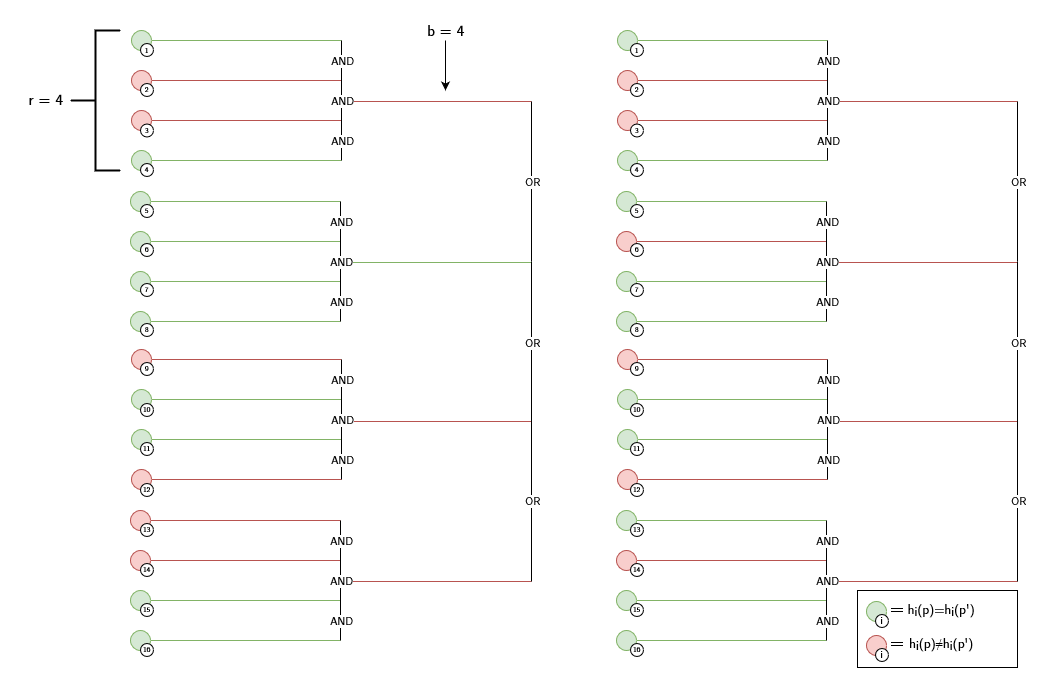
\includegraphics[width=\textwidth]{lsh_traditional_4.png}
    \caption[Visualization of two traditional LSH schemes with parameters $b=4$ and $r=4$]{\textbf{Visualization of two traditional LSH schemes with parameters $b=4$ and $r=4$}. The circles indicate an outcome of a hash function. A green circle indicates that the hash function agrees for $p$ and $p'$, while the opposite goes for a red circle.}
    \label{fig:lsh_traditional_visualization}
\end{figure}

\subsection{Parametrization of amplified LSH scheme}
An amplified LSH scheme uses exactly the same kind of operations (AND/OR) as a traditional LSH scheme, but applies them in an iterative way. In Figure \ref{fig:lsh_amplified_visualization} we take the input from the left visualized structure in Figure \ref{fig:lsh_traditional_visualization} and feed it to an amplified LSH scheme. In stage $1$ of the scheme we find groups of $r_1$ hash functions, connected by AND operators. Contrary to traditional LSH schemes, we do not connect all resulting signals with OR operators, but we create groups of signals. Each of these groups contains $b_1$ signals. This means that the number of resulting signals from stage $1$ is equal to $\frac{n}{b_1 * r_1}$. In the visualized structure, this amounts to $\frac{16}{2*2} = 4$ signals. In stage $2$ of the scheme, we again apply AND and OR operations. In this example, we group the signals in number of $b_2 = 2$ groups of $r_2 = 2$ signals. Following the rules laid down earlier, this specific amplified LSH scheme would consider $(p, p')$ not to be a candidate pair.

\begin{figure}[h!]
    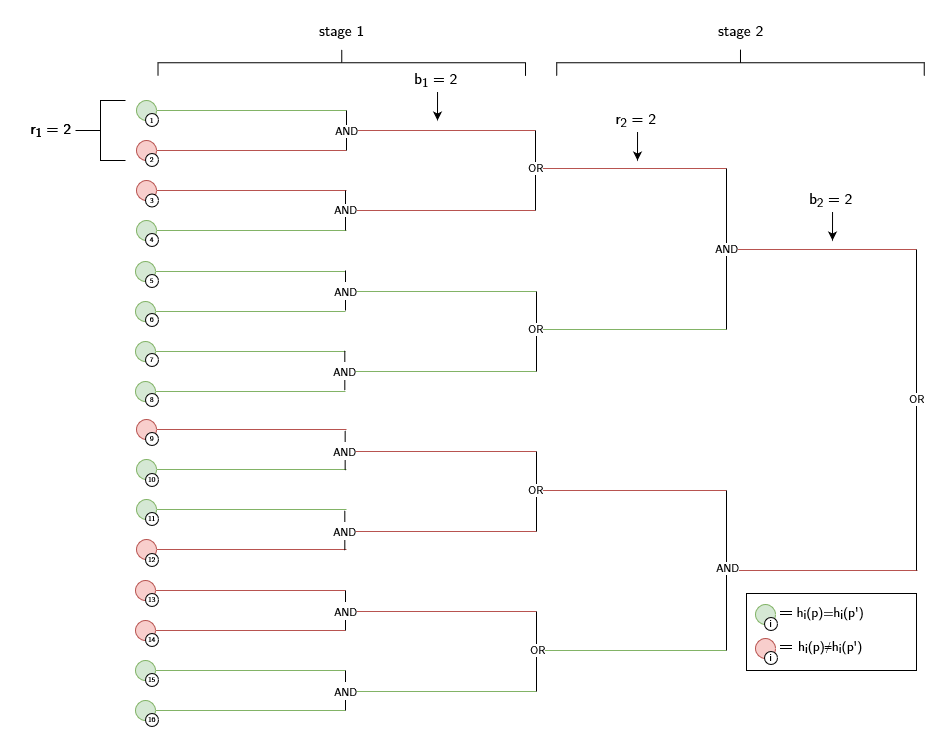
\includegraphics[width=\textwidth]{lsh_amplified_4.png}
    \caption[Visualization of an amplified LSH scheme with parameters $r_1=2$, $b_1=2$, $r_2=2$ and $r_2=2$]{\textbf{Visualization of an amplified LSH scheme with parameters $r_1=2$, $b_1=2$, $r_2=2$ and $r_2=2$}}
    \label{fig:lsh_amplified_visualization}
\end{figure}

How do essential properties of the amplified LSH scheme then compare to the traditional scheme? Using the parametrization described in the previous paragraph, we move our attention to the construction of the s-curve, the function that gives the probability of assigning $(p,p')$ as a candidate pair given the actual similarity of $p$ and $p'$. Given $s(p, p') = s$, we know that the probability of a positive signal in a group of $r_1$ hash function in stage $1$ is equal to $s^{r_1}$, which sets the probability of a negative signal equal to $1 - s^{r_1}$. Hence, the probability that $b_1$ of these groups all produce a negative signal is equal to $(1-s^{r_1})^{b_1}$. To conclude the first stage, the probability that there is a positive signal in at least one of the groups is equal to $1 - (1-s^{r_1})^{b_1}$. Some might notice the strong similarity of this formula to the formula of the original s-curve in equation \ref{eq:s_curve}. This should not be a surprise, as stage $1$ can be considered to consist of a number of $\frac{n}{b_1 * r_1}$ traditional LSH schemes, with parameters $b=b_1$ and $r=r_1$.

Moreover, stage $2$ is actually a traditional LSH scheme as well, with parameters $b=b_2$ and $r=r_2$. In the previous paragraph we have found that each of the input signals to stage $2$ has a probability of  $1 - (1-s^{r_1})^{b_1}$ of being positive. Using the two aforementioned facts, we can construct the formula for the s-curve of an amplified LSH scheme by substituting the probability of a stage $1$ signal being positive into the formula of the original s-curve related to stage $2$

\begin{align}
    Pr[(p, p')\text{ is a candidate pair}] &= 1 - (1- Pr[\text{positive input signal}]^{r_2})^{b_2} \\
                                           &= 1 - (1- (1 - (1-s^{r_1})^{b_1})^{r_2})^{b_2} \nonumber
    \label{eq:amplified_s_curve}
\end{align}

\subsection{Analysis of properties of amplified LSH scheme}
The s-curve allows us to analyze theoretical properties of the $(r_1,b_1,r_2,b_2)$-amplified LSH scheme. First, we might try to find an expression for the threshold $t$, so that we can relate $t$ to the parameters $(r_1,b_1,r_2,b_2)$, just like we do for the traditional LSH scheme in Equation \ref{eq:threshold_equation}. Again, like in Section \ref{section:lit:introducing_lsh}, we could try to solve 
\begin{equation}
    \frac{\partial^2 1 - (1- (1 - (1-s^{r_1})^{b_1})^{r_2})^{b_2} }{\partial s^2} = 0
    \label{eq:identifying_equation_amplified}
\end{equation}
 Via complex derivations, which can be found in Appendix \ref{appendix:derivation_second_derivative_s_curve}, we arrive at the expression below.
\begin{equation}
    \begin{aligned}
        &{r_1}^{2} {b_1}^{2}({r_2}-1) {r_2} {b_2} s^{2 {r_1}-2}\gamma^{2 {b_1}-2}\beta^{{r_2}-2}\alpha^{{b_2}-1} + ({r_1}-1) {r_1} {b_1} {r_2} {b_2} s^{{r_1}-2}\gamma^{{b_1}-1}\beta^{{r_2}-1}\alpha^{{b_2}-1}  = \\
        &{r_1}^{2} {b_1}^{2} {r_2}^{2}({b_2}-1) {b_2} s^{2 {r_1}-2}\gamma^{2 {b_1}-2}\beta^{2 {r_2}-2}\alpha^{{b_2}-2} + {r_1}^{2}({b_1}-1) {b_1} {r_2} {b_2} s^{2 {r_1}-2}\gamma^{{b_1}-2}\beta^{{r_2}-1}\alpha^{{b_2}-1} \\ 
        &\Leftrightarrow\\
        & {r_1}^{2} {b_1}^{2}({r_2}-1) {r_2} {b_2} s^{r_1}\gamma^{{b_1}-1}\beta + ({r_1}-1) {r_1} {b_1} {r_2} {b_2} s^{{r_1}-2}\gamma^{{b_1}-1}\beta^{{r_2}-1}\alpha^{{b_2}-1} = \\
        & {r_1}^{2} {b_1}^{2} {r_2}^{2}({b_2}-1) {b_2} s^{r_1}\gamma^{{b_1}-1}\beta^{{r_2}-1}\alpha + {r_1}^{2}({b_1}-1) {b_1} {r_2} {b_2} s^{r_1}\gamma\\
        &\text{with } \alpha = (1 - (1- (1 - s^{r_1})^{b_1})^{r_2} \\
        &\text{     } \beta = 1- (1 - s^{r_1})^{b_1}\\
        &\text{     } \gamma = 1 - s^{r_1} 
    \end{aligned}
\end{equation}
Unfortunately, we are not able to simplify this expression any further such that we obtain an analytical solution for the relationship between threshold $t$ and parameters $(r_1,b_1,r_2,b_2)$ in the amplified LSH scheme. 

The other route for obtaining a set of optimal parameter values is by minimizing the weighted average of the probability of false negative and the probability of false positives. These probabilities are given by  
\begin{equation}
    \begin{aligned}
        Pr[\text{False positive}] &= Pr[(x, y)\text{ is a candidate pair}| s(x, y) < t ] \\
                                  &= \int_{0}^{t}1 - (1- (1 - (1-s^{r_1})^{b_1})^{r_2})^{b_2}ds \\
                                  &= f(t,b_1,r_1,b_2,r_2) \\
        Pr[\text{False negative}] &= Pr[(x, y)\text{ is not a candidate pair}| s(x, y) > t ] \\
                                  &= \int_{t}^{1}1 - (1 - (1- (1 - (1-s^{r_1})^{b_1})^{r_2})^{b_2})ds \\
                                  &= g(t,b_1,r_1,b_2,r_2) \\
    \end{aligned}
    \label{eq:amplified_version_of_prob_neg_pos}
\end{equation}

Minimizing the weighted average of $ Pr[\text{False positive}]$ and $Pr[\text{False negative}]$ is then equivalent to solving the following problem, where we minimize $z(b_1,r_1,b_2,r_2| w_{FP}, w_{FN}))$

\begin{equation}
    \argmin_{b_1,r_1,b_2,r_2}  z(b_1,r_1,b_2,r_2| w_{FP}, w_{FN}))) = w_{FP} *  \int_{0}^{t}f(t,b_1,r_1,b_2,r_2)bds + w_{FN} * \int_{t}^{1}g(t,b_1,r_1,b_2,r_2)ds
    \label{eq:optimization_amplified}
\end{equation}

What happens to the amplified s-curve if we set $r_2=b_2=1$? 
\begin{equation}
    \begin{aligned}
    1 - (1- (1 - (1-s^{r_1})^{b_1})^{r_2})^{b_2} &= 1 - (1- (1 - (1-s^{r_1})^{b_1})^{1}
    )^{1} \\
    &= 1 - 1 + 1 -(1-s^{r_1})^{b_1}\\
    &= 1 - (1-s^{r_1})^{b_1}
    \end{aligned}
\end{equation}
This form is exactly equal to the traditional s-curve. Now, let $b_1=\hat{b}$ and $r_1=\hat{r}$, where $\hat{b}$ and $\hat{r}$ are solutions to the optimization problem in Equation \ref{eq:optimize_for_b_and_r}. Then the parameter configuration $(r_1,b_1,r_2,b_2) = (\hat{r}, \hat{b},1,1)$ gives a solution for the optimization problem in Equation \ref{eq:optimization_amplified} that is equal to the optimal solution to Equation \ref{eq:optimize_for_b_and_r}, the traditional LSH scheme. Hence, we have shown that it is always possible to find a configuration of parameters for the amplified LSH scheme that works as least as good as the traditional LSH scheme. By evaluating $z(b_1,r_1,b_2,r_2| w_{FP}, w_{FN}))$ for other values of $(r_1,b_1,r_2,b_2)$, we might find configurations of the amplified LSH scheme that improve on the traditional LSH scheme, keeping $n$ constant.

\subsection{Finding optimal parameter values for (amplified) LSH scheme}
In order to find optimal parameter values for $(r_1,b_1,r_2,b_2)$, we do an exhaustive search over all possible combinations of parameter values for a given number $n$ of hash functions $h_i(.)$, threshold $t$ and assumed weights $w_{FP}$ and $w_{FN}$. We set $w_{FP} = w_{FN} = 0.5$. This search is in Algorithm \ref{alg:optimize_lsh_paramaters}. The algorithm can be applied in  the amplified as well as the non-amplified setting. The algorithm introduces a new parameter $b_0$, which represents the total number of groups of $r_1$ hash functions in the first layer. The maximum value of $b_0$ is equal to $\lfloor \frac{n}{r_1} \rfloor$, while the minimum value of $b_0$ is $1$.

We apply Algorithm \ref{alg:optimize_lsh_paramaters} to find optimal parameters for all configurations $(n, t, a) \in N\times T \times A$, where the sets $N$, $T$, and $A$ are defined as 
\begin{equation}
    \begin{aligned}
        N &= \{16, 32, 64,128, 256, 512, 1024\} \\
        T &= \{0.05,0.1,0.15,0.2,0.25,0.3,0.35,0.4,0.45,0.5,0.55,0.6,0.65,0.7,0.75,0.8,0.85,0.9,0.95\}\\
        A &= \{\text{amplified}, \text{not amplified}\}
    \end{aligned}
    \label{eq:possible_parameters}
\end{equation}
This makes for a total of $|N|*|T|*|A| = 6 * 19 * 2 = 228 $ configurations.
\begin{algorithm}
    % \KwData{}
    \KwIn{\\
    $t$: Threshold value\\
    $n$: Number of hash functions \\
    $w_{FP}$: False positive weight\\
    $w_{FN}$: False negative weight \\
    $amplified$: Boolean variable that indicates whether we are allowing an amplified LSH scheme (multiple layers) \\
    $getFactors(x)$: Function that returns the set of all factors of $x$, including $1$ and $x$ \\
    $f(t,r_1,b_1,r_2,b_2)$,$g(t,r_1,b_1,r_2,b_2)$: Functions as defined in Equation \ref{eq:amplified_version_of_prob_neg_pos}}

    \KwResult{ A set of optimized parameters $r_{1}^{opt}, b_{1}^{opt}, r_{2}^{opt},b_{2}^{opt}$ for an amplified LSH scheme}
    $\epsilon_{min} \gets \infty$\;
    $b_{1}^{opt}, b_{2}^{opt},r_{1}^{opt},r_{2}^{opt} \gets 0,0,0,0$\;
    \For{$r_1 = 1; r_1 < n; r_1 = r_1 - 1$}{
    
        $max\_b_0 \gets \lfloor \frac{n}{r_1} \rfloor$\;
        \For {$b_0 = max\_b_0 ;b_0 > 0; b_0 = b_0 - 1$} {
        
            \uIf{$amplified$}{
                $b_1\_options \gets getFactors(b_0)$\;
            }
            \Else{
                $b_1\_options \gets \{b_0\}$\;
            }
            \For{$b_1 \textbf{ in } b_1\_options $}{
                $n_2 \gets \lfloor \frac{b_0}{b_1} \rfloor$ \;
                
                \uIf{$amplified$}{
                    $b_2\_options \gets getFactors(n_2)$\;
                }
                \Else{
                    $b_2\_options \gets \{1\}$\;
                }
                \For{$b_2 \textbf{ in } b_2\_options $}{
                    $r_2 \gets \lfloor \frac{n_2}{b_2} \rfloor$\;
                    $fp \gets f(t,b_1,r_1,b_2,r_2)$\;
                    $fn \gets g(t,b_1,r_1,b_2,r_2)$\;
                    $\epsilon \gets w_{FP} * fp + w_{FN} * fn$\;
                    \uIf{$\epsilon < \epsilon_{min}$} {
                        $\epsilon_{min} \gets \epsilon$\;
                        $r_{1}^{opt} \gets r_1$\;
                        $b_{1}^{opt} \gets b_1$\;
                        $r_{2}^{opt} \gets r_2$\;
                        $b_{2}^{opt} \gets b_2$\;
                    }
                }
            }
        }
    }
    \KwRet{$r_{1}^{opt}, b_{1}^{opt},r_{2}^{opt},b_{2}^{opt}$}
    \caption{Optimze LSH parameters}
    \label{alg:optimize_lsh_paramaters}
    \end{algorithm}
    
\subsection{Technical implementation details of amplified LSH scheme}
We extend the datasketch \footnote{available at https://github.com/ekzhu/datasketch} LSH scheme implementation, and create a new class LSHAmplified. This class is largely modeled after the original MinHashLSH class from the same package. Just like MinHashLSH, a list of hash tables is used as a data storage structure to allow the scheme to efficiently query points. The keys in each hash table have a length of $r_1$. While the traditional LSH implementation uses $b$ hash tables, the total number of hash tables in LSHAmplified is equivalent to $r_2 * b_1 * b_2$. The most notable difference between the two approaches is found in the method of extracting candidate pairs.

\subsubsection{Extracting candidate pairs from amplified LSH scheme}
The traditional LSH scheme extracts candidate pairs by looping over the hash tables and extracting elements that share a key in one of the hash tables. This simple approach unfortunately cannot be carried over, due to the more complex structure of the amplified LSH scheme. We propose and implement a new method of extracting candidate pairs in Algorithm \ref{alg:extract_candidate_pairs_amplified_abstract}. In the next paragraph, we go through the key steps in the algorithm.

To understand the algorithm, it helps to first look at the the second stage. Take for example the amplified scheme as pictured in Figure \ref{fig:lsh_amplified_visualization}. Due to the final OR-construction in the second stage, we find that we can separately check whether the AND/OR-constructions linked to the top $8$ hash functions or those linked to the bottom $8$ hash functions produce a positive signal. Hence, in our algorithm we start wih a loop over the number of bands $b_2$ in the second stage, after initiating an empty set $C$, which will contain the candidate pairs after completion of the algorithm.

Per band, we create a map $candidates\_per\_group$ of length $r_2$.  We then iterate through all the hash tables that belong to that band. Per hashtable, we extract all pairs of duplicates that share a key and store the pair in $candidates\_per\_group[cur\_group]$. $cur\_group$ refers to the specific group of AND/OR constructions in that the hash table belongs to in the first stage. There are $r_2$ of such groups per band. Finally, we loop through $candidates\_per\_group$ and extract the pairs that are found in all values of $candidates\_per\_group$. These pairs are are added to $C$. After the outer loop over all bands $b_2$ has completed, $C$ contains the candidate pairs.

%In LSHAmplified, we take the following steps to extract the candidate pairs. We initialize a dictionary named $candidate\_pairs\_per\_group$ with a total of $b_2 * r_2$ keys. The initial value of each key is an empty set. Each key corresponds to $1$ input to the second stage of the amplified scheme. In the example in figure \ref{fig:lsh_amplified_visualization}, there would be $4$ of such groups. We now loop through the list of hash tables. From each hash table $j$, we extract all points $p$ that have the same hash code $g_j(p)$ and create the set of all pairs $\{(p, p'): g_j(p)==g_j(p'), p \neq p'\}$. All pairs in the set are then added to the set belonging to the key $int(\frac{j}{b_1})$ in $candidate\_pairs\_per\_group$. 

%After this operation we have obtained the candidate pairs per group of $r_1$ rows and $b_1$ bands in the first layer. We initialize an empty set named $candidate\_pairs$ We set-up a second loop, that iterates through the bands in the second stage. Per band $k \in [b_2]$, we gather all candidate pairs that are found in every group in the band. Those candidate pairs are added to $candidate\_pairs$. After this operation, $candidate\_pairs$ contains all candidate pairs from the amplified LSH scheme.

% \begin{algorithm}
%     \KwData{\\
%     $L$: List of hash tables $H$\\}
%     \KwIn{\\
%     $(b_1,r_1,b_2,r_2)$: parameters of (amplified) LSH scheme \\}
%     \KwResult{ A set of candidate pairs $C$}
%     $C \gets \{\}$\;
%     \For{$i = 1; i \leq b_2; i = i + 1$}{
%         $candidates\_per\_group \gets Map<key, value>$\;
%         \For{$j = 1; j \leq r_2; i = i + 1$}{
%            $candidates\_per\_group[j] \gets \{\}$\;
%         }
%         \For {$H \textbf{ in } L[(i - 1)r_{2}b_{1}:ir_{2}b_{1}]$} {
%             $cur\_group \gets \lfloor \frac{H.index}{b_1} \rfloor$\;
%             \For{$key \textbf{ in } H$}{                
%                 \uIf{$length(H[key]) > 1$}{
%                     $pairs \gets \text{Set of all pairs in $H[key]$}$\;
%                     $candidates\_per\_group[cur\_group] \gets candidates\_per\_group[cur\_group] \bigcup pairs  $\;
%                 }
%             }
%         }
%         $candidate\_pair\_counter \gets Map<key, value>$\; 
%         \For{$j = 0; j \leq r_1; j = j + 1$}{
%             \For{$cp \textbf{ in } candidates\_per\_group[j]$}{
%                 $candidate\_pair\_counter[cp] \gets candidate\_pair\_counter[cp] + 1$\;
%             }
%         }
%         \For{$cp \textbf{ in } candidate\_pair\_counter $}{
%             \uIf{$candidate\_pair\_counter[cp] == r_2$}{
%                 $C \gets C \bigcup cp$
%             }
%         }
%     }
%     \KwRet{$C$}
%     \caption{Extract candidate pairs from amplified LSH scheme}
%     \label{alg:extract_candidate_pairs_amplified}
%     \end{algorithm}

\begin{algorithm}
        \KwData{\\
        $L$: List of hash tables $H$\\}
        \KwIn{\\
        $(b_1,r_1,b_2,r_2)$: parameters of (amplified) LSH scheme \\}
        \KwResult{ A set of candidate pairs $C$}
        $C \gets \{\}$\;
        \For{$i = 1; i \leq b_2; i = i + 1$}{
            $candidates\_per\_group \gets \text{Empty Map of length $r_2$} $\;
            //Loop through $L$ starting on index $(i - 1) * r_{2} *b_{1}$ until index $i* r_{2} *b_{1}$\;
            \For {each hash table $H$ in $L[(i - 1)r_{2}b_{1}:ir_{2}b_{1}]$} {
                $j \gets \lfloor \frac{H.index}{b_1} \rfloor$\;
                Extract all pairs from H into $candidates\_per\_group[j]$\;
            }
            \For {each pair $cp$ extracted}{           
                \uIf{$cp$ in every entry of $candidates\_per\_group$}{
                    $C \gets C \bigcup cp$\;
                }
            }
        }
        \KwRet{$C$}
        \caption{Extract candidate pairs from amplified LSH scheme (abstract version)}
        \label{alg:extract_candidate_pairs_amplified_abstract}
\end{algorithm}
        
    
\section{Evaluation of LSH schemes}
\label{section:meth:evaluation_lsh_schemes}

Following the standard in literature, we evaluate the LSH scheme by three effectiveness measures: the pair completeness (PC), pair quality (PQ), and reduction ratio (RR). The PC is defined as follows:
\begin{equation}
    PC = \frac{D_f}{D_n}
    \label{eq:formula_pair_completeness}
\end{equation}
where $D_f$ refers to the number of true duplicates found and $D_n$ refers to the total number of true duplicates. In both instances we refer to pairwise duplicates. Hence, if an entity is found in four different webshops, it contributes a total of $6$ pairwise duplicates to $D_n$. 

The PQ is defined as follows:
\begin{equation}
    PQ = \frac{D_f}{N_c}
    \label{eq:formula_pair_quality}
\end{equation}
where $N_c$ refers to the number of duplicates found. $N_c$ is the result of taking the candidate pairs returned by the LSH scheme of interest and filtering out all candidate pairs that are from the same shop or the same brand, since we know for sure that those pairs are not duplicates.

Lastly, we define the the RR as:
\begin{equation}
    RR = 1 - \frac{N_c}{N_{ac}}
    \label{eq:formula_reduction_ratio}
\end{equation}
where $N_{ac}$ refers to the total number of available comparisons in the data, again corrected for brand and shop.

In our evaluations of methods, we are interested in (configurations of) methods that simultaneously score high for $PC$ and $RR$. Such methods automatically score high for $PQ$ as well. $PQ = \frac{D_f}{N_c} = \frac{PC * D_n}{(1-RR)N_{ac}}$ implies that any method that improves at least one of $PC$ and $RR$ and does not decrease the other will also see an increase in $PQ$. Furthermore, as described in Section \ref{section:lit:deduplication_in_hhs}, based on $PC$ and $RR$, we can define the measure $\alpha$, which serves as a general measure for the effectiveness of a LSH scheme

\begin{equation}
    \alpha = PC * RR
\end{equation}

We evaluate these measures for the configurations as defined in Equation \ref{eq:possible_parameters}. In order to get a consistent estimate of the measures, we run a bootstrap evaluation with $25$ iterations. In each iteration, we randomly select $\frac{2}{3}$ of the dataset to apply the methods too. The final estimated values of the measures are then calculated by taking the average of the measure over the $25$ iterations per configuration ($n$,$t$,$a$).

